\documentclass[12pt, twoside]{article}
\usepackage[letterpaper, margin=1in, head=30pt, headsep=0.1in]{geometry}
\usepackage[english]{babel}
\usepackage[utf8]{inputenc}
\usepackage{amsmath}
\usepackage{amsfonts}
\usepackage{amssymb}
\usepackage{tikz}
\usetikzlibrary{quotes, angles}

\usepackage{graphicx}
\usepackage{enumitem}
\usepackage{multicol}

%\usepackage{pgfplots}
%\pgfplotsset{width=10cm,compat=1.9}
%\usepgfplotslibrary{statistics}
%\usepackage{pgfplotstable}
%\usepackage{tkz-fct}
%\usepackage{venndiagram}

\usepackage{fancyhdr}
\pagestyle{fancy}
\fancyhf{}
\renewcommand{\headrulewidth}{0pt} % disable the underline of the header
\raggedbottom
\newif\ifmeta
\metatrue %print standards and topics tags

\title{Math AI Worksheet Generator and Formative Assessment System}
\author{Chris Huson}
\date{November 2020}

%\fancyhead[RE]{\thepage}
%\fancyhead[RO]{\thepage \\ Name: \hspace{3cm}}
%\fancyhead[L]{BECA / Dr. Huson / 10th Grade Geometry\\* 7 June 2019}
%
%\begin{document}
%\subsubsection*{13.7 Homework: Cross sections, distance applications}
%\fancyhead[L]{BECA / Dr. Huson / Geometry 03-Volume+angle-bisectors\\* pset ID: 34}

\begin{document}

\subsubsection*{3.10 Solving for dimensions given a volume}
\begin{enumerate}

\item Do Now: Find the volume of a rectangular prism (box). Its length is $l=10$ feet, its height $h=4$, and depth is $w=3$ feet. Start with the equation \\[0.5cm]
$V = l \times w \times h$
  \begin{flushright}
    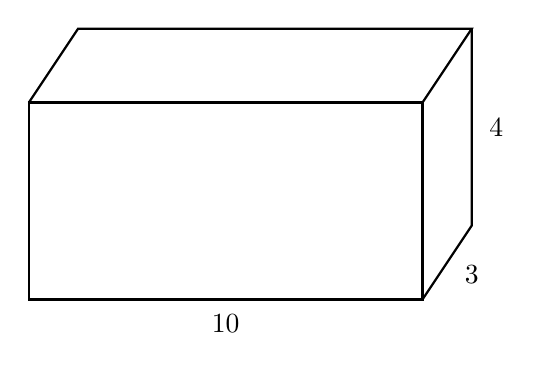
\begin{tikzpicture}[scale=1.25]
      \draw [-, thick] (0,0)--(4,0)--(4,2)--(0,2)--cycle;
      \draw [-, thick] (0,2)--(0.5,2.75)--(4.5,2.75)--(4,2);
      \draw [-, thick] (4,0)--(4.5,0.75)--(4.5,2.75);
      \node at (4.75, 1.75){$4$};
      \node at (2, -0.25){$10$};
      \node at (4.5, 0.25){$3$};
    \end{tikzpicture}
  \end{flushright}
  
\newpage
\item Rectangle $ABCD$ has area $A=15$ and base $b=6$ but unknown height. Write an equation then solve. Start with this form (for the unknown, use $h$, $x$, or $BC$) and state your answer as a fraction: \\[0.5cm]
$A = b \times h = 15$
  \begin{flushright}
  \begin{tikzpicture}[scale=1.25]
    \draw [-, thick] (0,0)--(4.5,0)--(4.5,2)--(0,2)--cycle;
    \draw [fill] (0,0) circle [radius=0.05] node[left]{$A$};
    \draw [fill] (4.5,0) circle [radius=0.05] node[right]{$B$};
    \draw [fill] (4.5,2) circle [radius=0.05] node[right]{$C$};
    \draw [fill] (0,2) circle [radius=0.05] node[left]{$D$};
    \node at (5, 1){?};
    \node at (2.25, -0.5){$6$};
    \node at (2.25, 1){$A = 15$};
  \end{tikzpicture}
  \end{flushright}

\newpage
\item The $\triangle DEF$ has an area $A=54$ and base $DE=12$.
  \begin{multicols}{2}
    Find its height, starting with an equation. \\[0.5cm]
    $\displaystyle A = \frac{1}{2} bh = 54$ \vspace{2cm}
      \begin{flushright}
      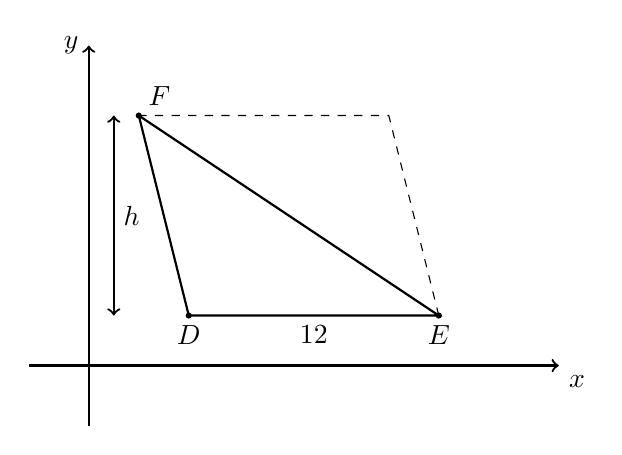
\begin{tikzpicture}[scale=.635]
        %\draw [help lines] (-1,-1) grid (9,6);
        \draw [thick, ->] (-1.2,0) -- (9.4,0) node [below right] {$x$};
        \draw [thick, ->] (0,-1.2)--(0,6.4) node [left] {$y$};
        \draw [<->, thick] (0.5,1)--(0.5,5);
        \draw [-, thick] (2,1)--(7,1)--(1,5)--cycle;
        \draw [-, dashed] (7,1)--(6,5)--(1,5);
        \draw [fill] (2,1) circle [radius=0.05] node[below] {$D$};
        \draw [fill] (7,1) circle [radius=0.05] node[below] {$E$};
        \draw [fill] (1,5) circle [radius=0.05] node[above right] {$F$};
        \node at (4.5,1)[below]{$12$};
        \node at (0.5,3)[right]{$h$};
      \end{tikzpicture}
      \end{flushright}
  \end{multicols}

\newpage
\item The volume of a rectangular prism (box) is $V=110$ cubic feet. Its height is $h=5$ feet and depth of $w=4$ feet. Find its length. Start with the equation \\[0.5cm]
$V = l \times w \times h = 110$
  \begin{flushright}
    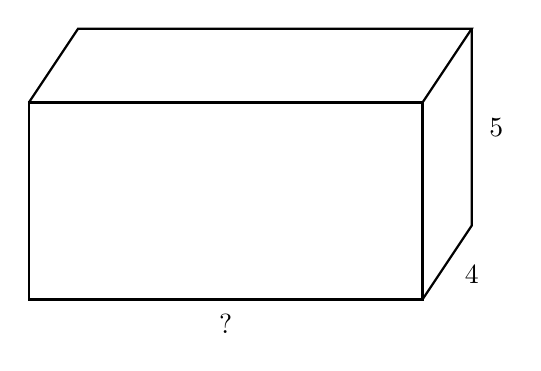
\begin{tikzpicture}[scale=1.25]
      \draw [-, thick] (0,0)--(4,0)--(4,2)--(0,2)--cycle;
      \draw [-, thick] (0,2)--(0.5,2.75)--(4.5,2.75)--(4,2);
      \draw [-, thick] (4,0)--(4.5,0.75)--(4.5,2.75);
      \node at (4.75, 1.75){$5$};
      \node at (2, -0.25){$?$};
      \node at (4.5, 0.25){$4$};
    \end{tikzpicture}
  \end{flushright}

\newpage
\item Find the length of the base of a triangle with area $A=78$ and height $h=20$. Express your result as a decimal. Start with the form (use $b$ or $x$): \\[0.5cm]
$A = \frac{1}{2} \times b \times h = 78$
  \begin{flushright}
  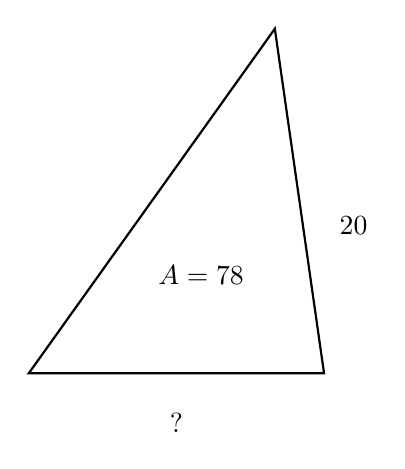
\begin{tikzpicture}[scale=1.25]
    \draw [-, thick] (0,0)--(3,0)--(2.5,3.5)--cycle;
    \node at (3.3, 1.5){20};
    \node at (1.5, -0.5){$?$};
    \node at (1.75, 1){$A = 78$};
  \end{tikzpicture}
  \end{flushright}

\newpage
\item Find the area of the given circle $Q$ with radius $r=10$ centimeters.
  \begin{multicols}{2}
  \raggedcolumns
  Start with the formula\\[0.5cm]
  $A = \pi r^2$ 
  \begin{enumerate}
    \item State the area in terms of $\pi$ \vspace{1.7cm}
    \item Now round to the nearest hundredth
  \end{enumerate}

    \begin{tikzpicture}[scale=1]
      \draw (0,0) circle[radius=3];
      \draw [thick]
      (0:3) node[right] {$P$}--
      (0,0) node[below] {$Q$};
      \draw (1.5,0) node[below] {$10$};
    \end{tikzpicture}
  \end{multicols}

\newpage
\item Given circle $O$ with area $r=49 \pi$ square centimeters.
  \begin{multicols}{2}
  \raggedcolumns
  Find the radius of circle, $OP$. Start with the formula\\[0.5cm]
  $A = \pi r^2 = 49 \pi$ \vspace{1.7cm}

    \begin{tikzpicture}[scale=1]
      \draw (0,0) circle[radius=3];
      \draw [thick]
      (0:3) node[right] {$P$}--
      (0,0) node[below] {$O$};
      \draw (1.5,0) node[below] {$?$};
    \end{tikzpicture}
  \end{multicols}

\newpage
\item Find the length of the base of a rectangle with area $A=22 \frac{1}{2}$ and height $h=5$, expressed as a fraction. Start with the form (use $b$ or $x$): \\[0.5cm]
$A = b \times h = 22 \frac{1}{2}$
  \begin{flushright}
  \begin{tikzpicture}[scale=1.25]
    \draw [-, thick] (0,0)--(3,0)--(3,3.5)--(0,3.5)--cycle;
    \node at (3.5, 2){5};
    \node at (1.5, -0.5){$?$};
    \node at (1.5, 2){$A = 22 \frac{1}{2}$};
  \end{tikzpicture}
  \end{flushright}
  
\end{enumerate}
\end{document}